% author Truong Nhan Nguyen

\documentclass[tikz, border=10pt]{standalone}

\usepackage{tikz}

% define commit styles
\tikzset{
    commit/.style = {draw=white, line width=1pt, circle},
    master/.style = {commit, fill=red, minimum size=1cm},
    hotfix/.style = {commit, fill=green, minimum size=0.9cm},
    develop/.style = {commit, fill=blue, minimum size=0.95cm},
    feature/.style = {commit, fill=magenta, minimum size=0.9cm},
    every label/.style = {rounded corners, inner sep=3pt, font=\sffamily\bfseries, text=white}
}

\begin{document}
    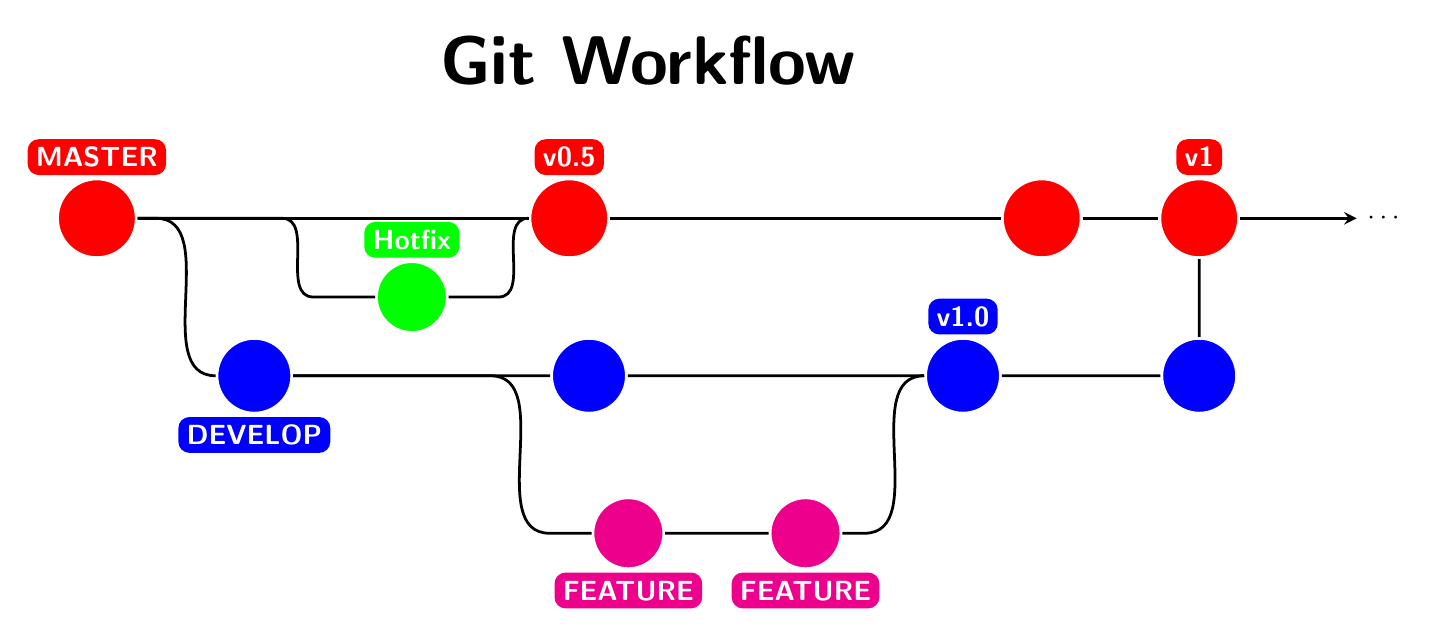
\begin{tikzpicture}[label distance=0.7pt]
        % place commit branchs
        \node[master, label={[fill=red]above:MASTER}] (master-1) at (0, 4) {};
        \node[develop, label={[fill=blue]-90:DEVELOP}] (develop-1) at (2, 2) {};
        \node[hotfix, label={[fill=green]above:Hotfix}] (hotfix-1) at (4, 3) {};
        \node[master, label={[fill=red]above:v0.5}] (master-2) at (6, 4) {};
        \node[develop] (develop-2) at (6.25, 2) {};
        \node[feature, label={[fill=magenta]below:FEATURE}] (feature-1) at (6.75, 0) {};
        \node[feature, label={[fill=magenta]below:FEATURE}] (feature-2) at (9, 0) {};
        \node[develop, label={[fill=blue]above:v1.0}] (develop-3) at (11, 2) {};
        \node[master] (master-3) at (12, 4) {};
        \node[master, label={[fill=red]above:v1}] (master-4) at (14, 4) {};
        \node[develop] (develop-4) at (14, 2) {};
        
        % draw master branch and hotfix branch
        \draw[line width=1pt, -stealth]
            (master-1) -- (master-2) -- (master-3) -- (master-4) -- (16, 4) node[right] {$\cdots$};
        \draw[line width=1pt] 
            (master-1) -- (2.35, 4) to[out=0, in=180] (2.75, 3) -- (hotfix-1) -- (5.1, 3) to[out=0, in=180] (master-2.west);
        % draw develop branch and feature branch
        \draw[line width=1pt]
            (master-1) -- (0.75, 4) to[out=0, in=180] (develop-1) -- (develop-2) -- (develop-3) -- (develop-4) -- (master-4);
        \draw[line width=1pt]
            (develop-1) -- (5, 2) to[out=0, in=180] (5.75, 0) -- (feature-1) -- (feature-2) -- (9.75, 0) to[out=0, in=180] (develop-3.west);
        % add title graphic
        \node[anchor=center] at (7, 6) {\Huge\bfseries\sffamily Git Workflow};
    \end{tikzpicture}
\end{document}